\newcommand{\deadline}{30.06.2023}

\documentclass[11pt]{article}

\usepackage[exercise,ex]{custom_2.1}

\begin{document}

\section{Magentfeldberechnung}
\begin{center}
    [siehe hinten]
\end{center} 

\section{Induktionsstrombremse}
\begin{align*}
    U_{ind} &= - \deriv{\phi}{t}\\
    &= - B \deriv{A}{t}\\
    &= - B d v\\
    I_{ind} &= \frac{U_{ind}}{R}\\
    &= - \frac{B d v}{R}\\
    \\
    0 &= \Delta W_{pot} + \Delta W_{kin} + \Delta W_{el}\\
    0 &= m g x + \frac m2 v^2 + \int I_{ind} U_{ind} \dt\\
    0 &= m g x + \frac m2 v^2 + \frac{B^2 d^2 }{R} \int v^2 \dt\\
    0 &= m g v + m v a + \frac{B^2 d^2 }{R} v^2 \\
    a &= - g - \frac{B^2 d^2 }{m R} v \\
    F_{ges} &= \underbrace{- m g}_{F_{g}} + \underbrace{ \frac{-B^2 d^2 }{R} v}_{F_{el}} \\
    \\
    v_{max} &\implies a=0 \\
    0 &= - g - \frac{B^2 d^2 }{m R} v_{max} \\
    v_{max} &= -g \frac{m R}{B^2 d^2}\\
    &\approx -\gravityearth \frac{45\u g \cdot4\,\Omega}{13^2 \u T^2 \cdot 15^2\u{cm}^2}\\
    &\approx 0.464 \ufrac{m}{s^2}
\end{align*}

\section{Ausschaltvorgang an einer Spule}
\begin{align*}
    0 &=  U_R + U_{ind}\\
    0 &=  I R + L \dot I\\
    0 &=  \dot I + \frac RL I \\
    I(t)  &= c \cdot e^{-\frac RL t}\\
    &= I_0 \cdot e^{-\frac RL t}
\end{align*}
\begin{adjustwidth}{20pt}{}
    Wobei \(I_0\) der Strom ist, der vor Entfernen der Spannungsquelle
    geflossen ist.
\end{adjustwidth}

\section{Dynamo}
\begin{figure}[h]
    \centering
    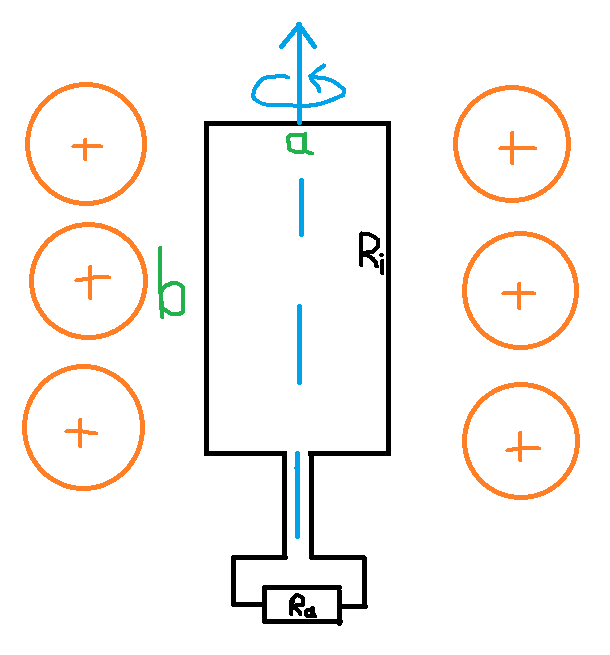
\includegraphics[width=0.5\textwidth]{1}
    \caption{Versuchsaufbau}
\end{figure}
\begin{align*}
    U_{ind} &= - N \deriv{\phi}{t}\\
    &= - N B \deriv A t\\
    &= - N B \deriv{}{t} \hug{ab \cos\varphi}\\
    &= - N B \deriv{}{t} \hug{ab \cos\hug{\omega t}}\\
    &= N ab B \omega \sin\hug{\omega t}\\
    I_{ind} &= \frac{N ab B \omega}{R_i+R_a} \sin\hug{\omega t}\\
    \\
    P_{mech} &= P_{el}\\
    M \omega &= \frac{U _{ind}^2}{R_{ges}}\\
    &= \frac{N^2 a^2b^2 B^2 \omega^2 \sin^2\hug{\omega t}}{R_{i} + R_a}\\
    M &= \frac{N^2 a^2b^2 B^2 \omega }{R_{i} + R_a} \sin^2\hug{\omega t}\\
    &\approx 250^2 \cdot 5^2\u{cm^2} \cdot 3^2\u{cm^2} \cdot  0.5^2\u T^2 \frac {\omega}{{R_{i} + R_a}}\sin^2\hug{\omega t}\\
    &\approx 3.52\cdot 10^{-2}\u{V\,s\,m^2} \frac {\omega}{{R_{i} + R_a}}\sin^2\hug{\omega t}\\
    \vec M &= \frac{N^2 a^2b^2 B^2 \omega}{R_{i} + R_a} \sin^2\hug{\omega t} \vec e_\omega \\
\end{align*}

\section{Nichtperiodische Fourierzerlegung}
\begin{align*}
    U(t) &= \begin{cases}
        0 \u V \ \ \ \te{für} &t<0 \u s\\
        U_0 \ \ \ \ \te{für} &0 \u s \le t \le t_0\\
        0\u V \ \ \ \te{für} &t_0< t\\
    \end{cases}
\end{align*}
\subsection{}
\begin{align*}
    F(U(t)\,;\,\omega) &= \int_{-\infty}^{\infty} U(t)\cdot e^{- i \omega t}\dt\\
    &= U_0 \int_{0}^{t_0} e^{- i \omega t}\dt\\
    &= -\frac{U_0}{i \omega}e^{- i \omega t}\eval_{0}^{t_0}\\
    &= \frac{U_0}{i \omega}\hug{1 - e^{- i \omega t_0}}\\
    &= \frac{i U_0}{\omega}\hug{e^{- i \omega t_0} - 1}\\
    &= \frac{i U_0}{\omega}\hug{\cos\hug{\omega t_0} - i\sin\hug{\omega t_0} - 1}\\
    \Re (F(U(t)\,;\,\omega)) &= \frac{U_0}{\omega}\sin\hug{\omega t_0} \ \ \bigl[= 2\pi\cdot  a(\omega )\bigr]\\
    \Im (F(U(t)\,;\,\omega)) &= \frac{U_0}{\omega}\hug{\cos\hug{\omega t_0} - 1} \ \ \bigl[= 2\pi\cdot  b(\omega )\bigr]\\
\end{align*}

\newpage
\subsection{}
\begin{figure}[h]
    \centering
    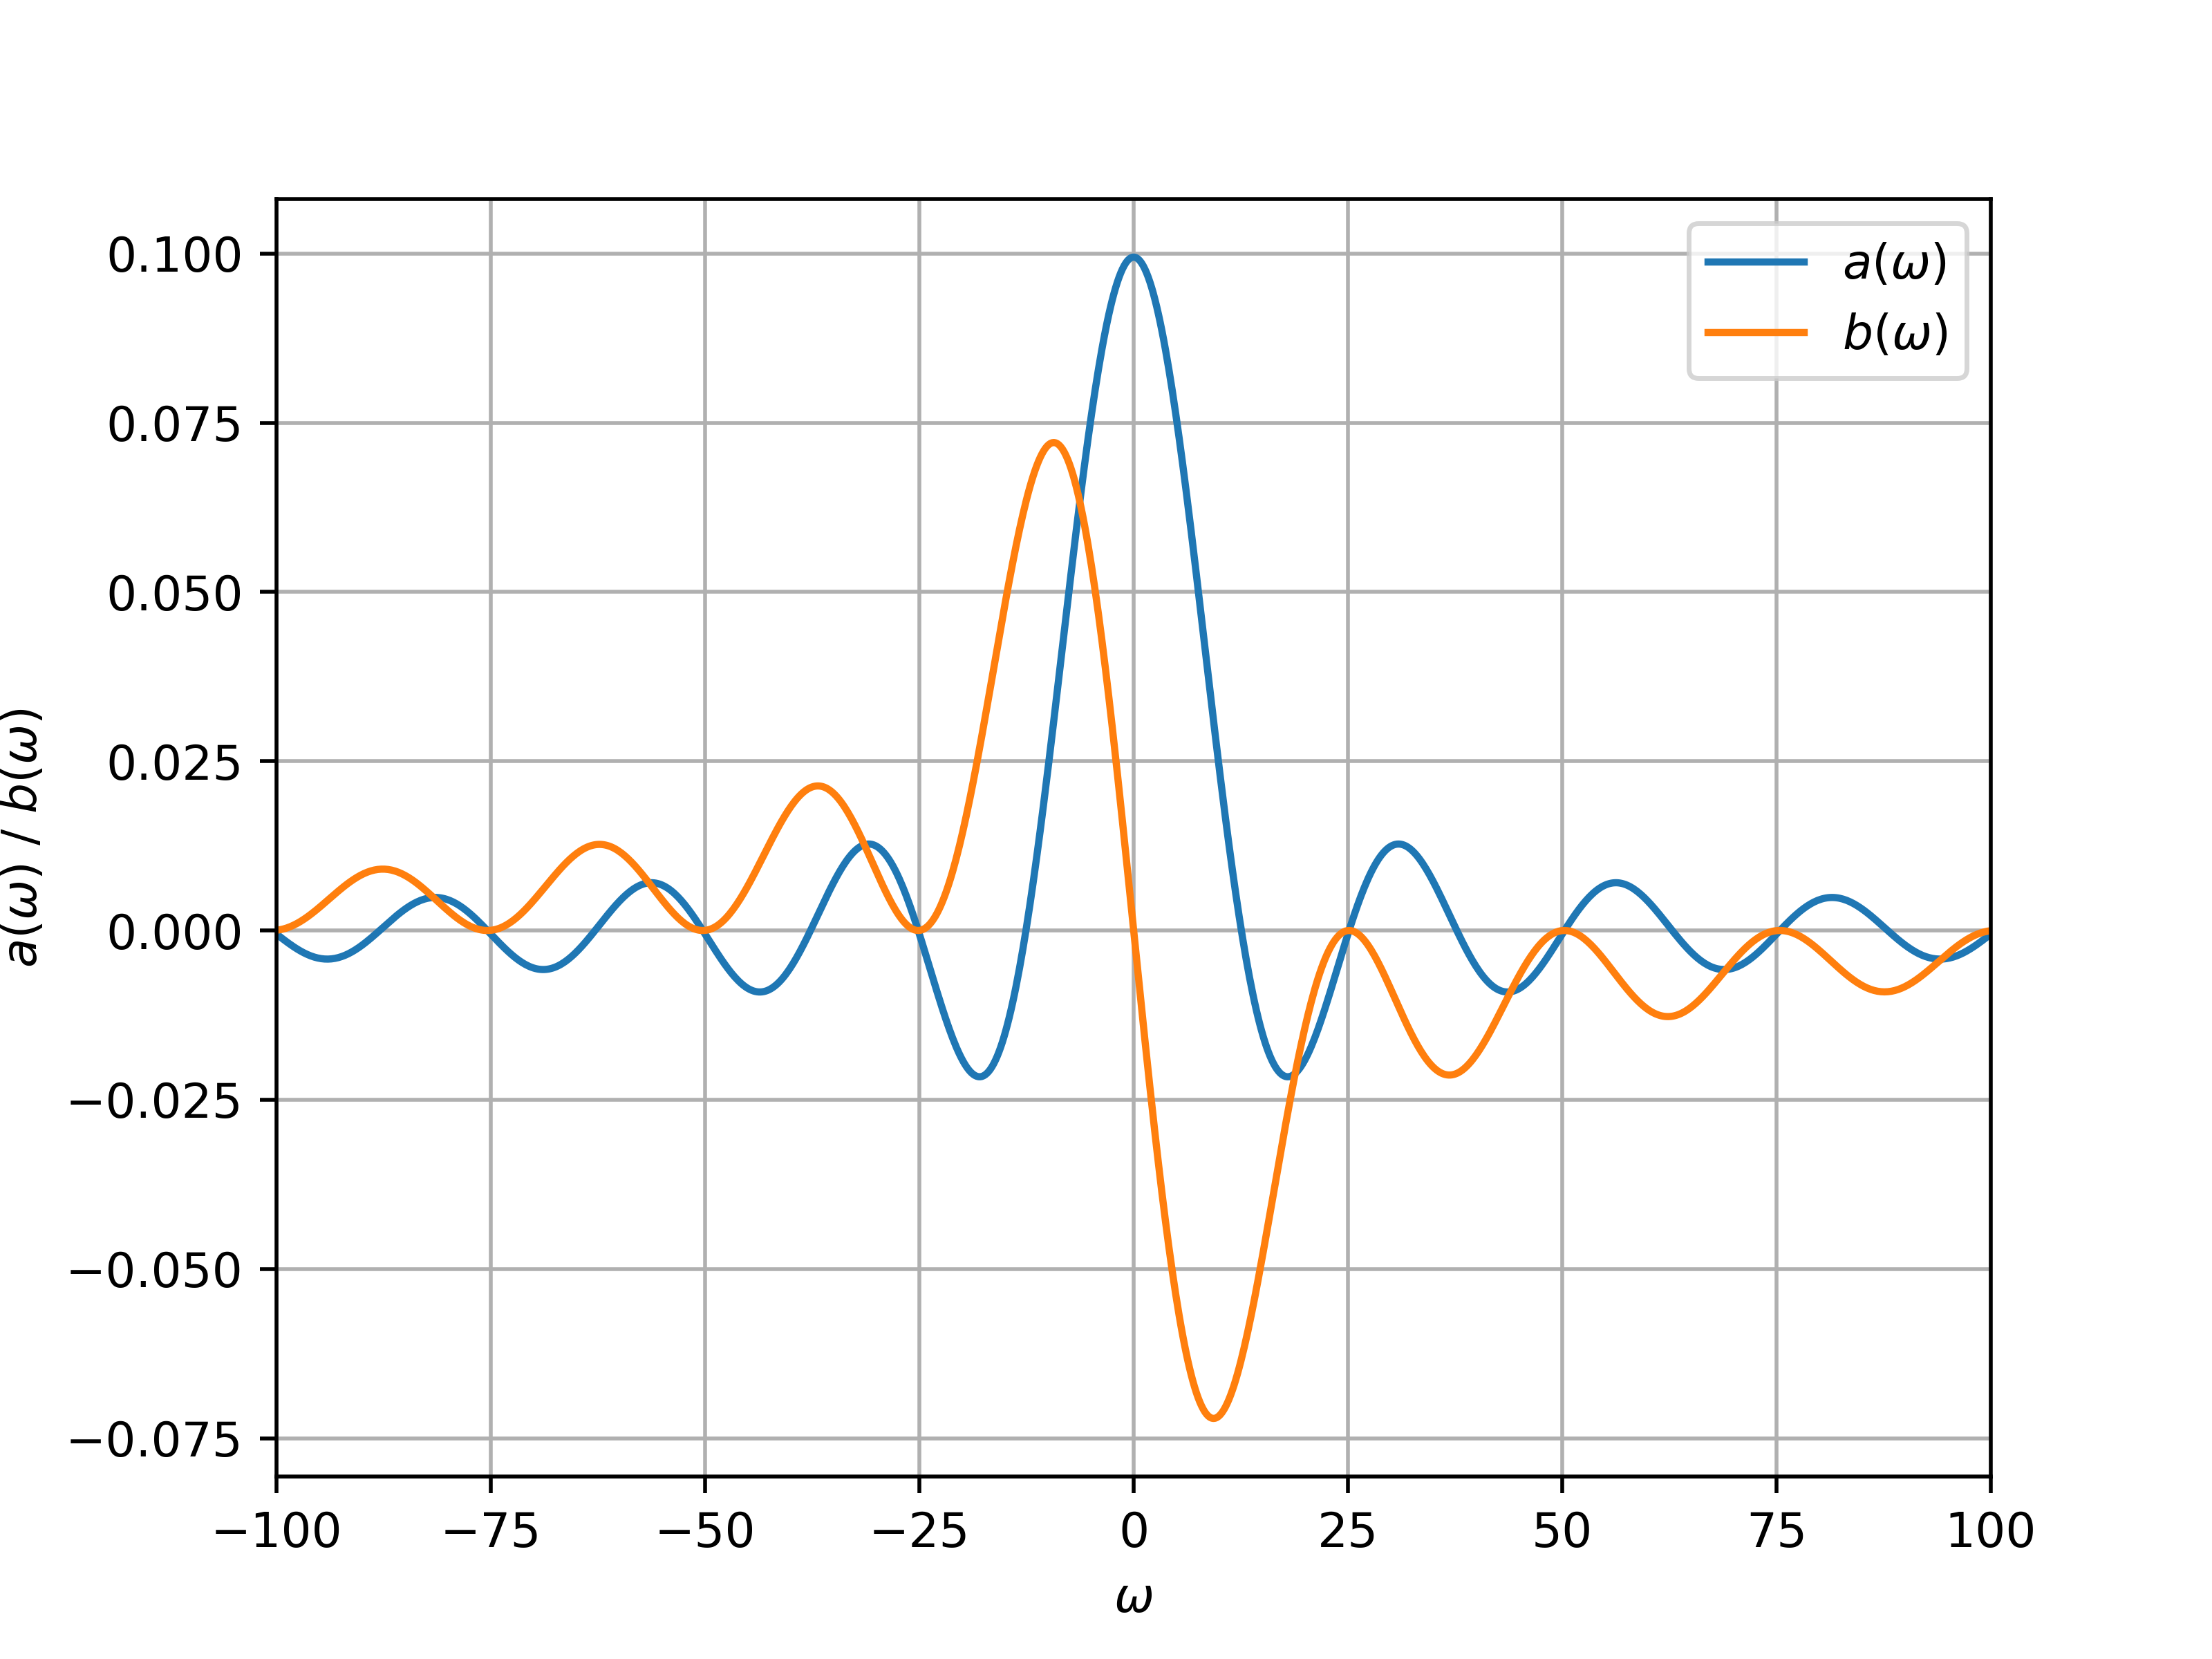
\includegraphics[width=0.7\textwidth]{5c.png}
    \caption{Plot von \(a(\omega)\) und \(b(\omega)\)}
\end{figure}

\subsection{}
\begin{align*}
    U(t) &= \int_{-\infty}^{\infty} \hug{\cos(\omega t) a(\omega) + \sin(\omega t) b(\omega)}\d\omega\\
    U(t) &= \frac{U_0}{2\pi}\int_{-\infty}^{\infty} \frac{\cos(\omega t)\sin (\omega t_0)}{\omega} + \frac{U_0}{2\pi}\int_{-\infty}^{\infty}\frac{\sin(\omega t)(\cos (\omega t_0)-1)}{\omega} \d\omega\\
    \int_{-\infty}^{\infty} \frac{\cos(\omega t)\sin (\omega t_0)}{\omega} &\eq 
    \frac 12 \pi (\sgn(t_0-t) + \sgn(t_0+t))\\
    \int_{-\infty}^{\infty}\frac{\sin(\omega t)(\cos (\omega t_0)-1)}{\omega} \d\omega
    &\eq -\frac 12 \pi (\sgn(t_0-t) - \sgn(t_0+t) + 2 \sgn(t))\\
    U(t) &= \frac{ U_0}{2\pi} \cdot \pi(\sgn(t_0 - t)+  \sgn(t))\\
    &= \frac{ U_0}{2}(\sgn(t_0 - t)+  \sgn(t))\\
    &= \begin{cases}
        0 \u V \ \ \ \te{für} &t<0 \u s\\
        U_0 \ \ \ \ \te{für} &0 \u s \le t \le t_0\\
        0\u V \ \ \ \te{für} &t_0< t\\
    \end{cases}
\end{align*}
\begin{adjustwidth}{20pt}{}
    \con Integral mit Wolfram Alpha, nachdem wir es zwei Stunden lang erfolglos selbst 
    versucht haben\\
    \con "
\end{adjustwidth}


\setcounter{section}{0}
\section{Magentfeldberechnung}
\doublesubsection{}
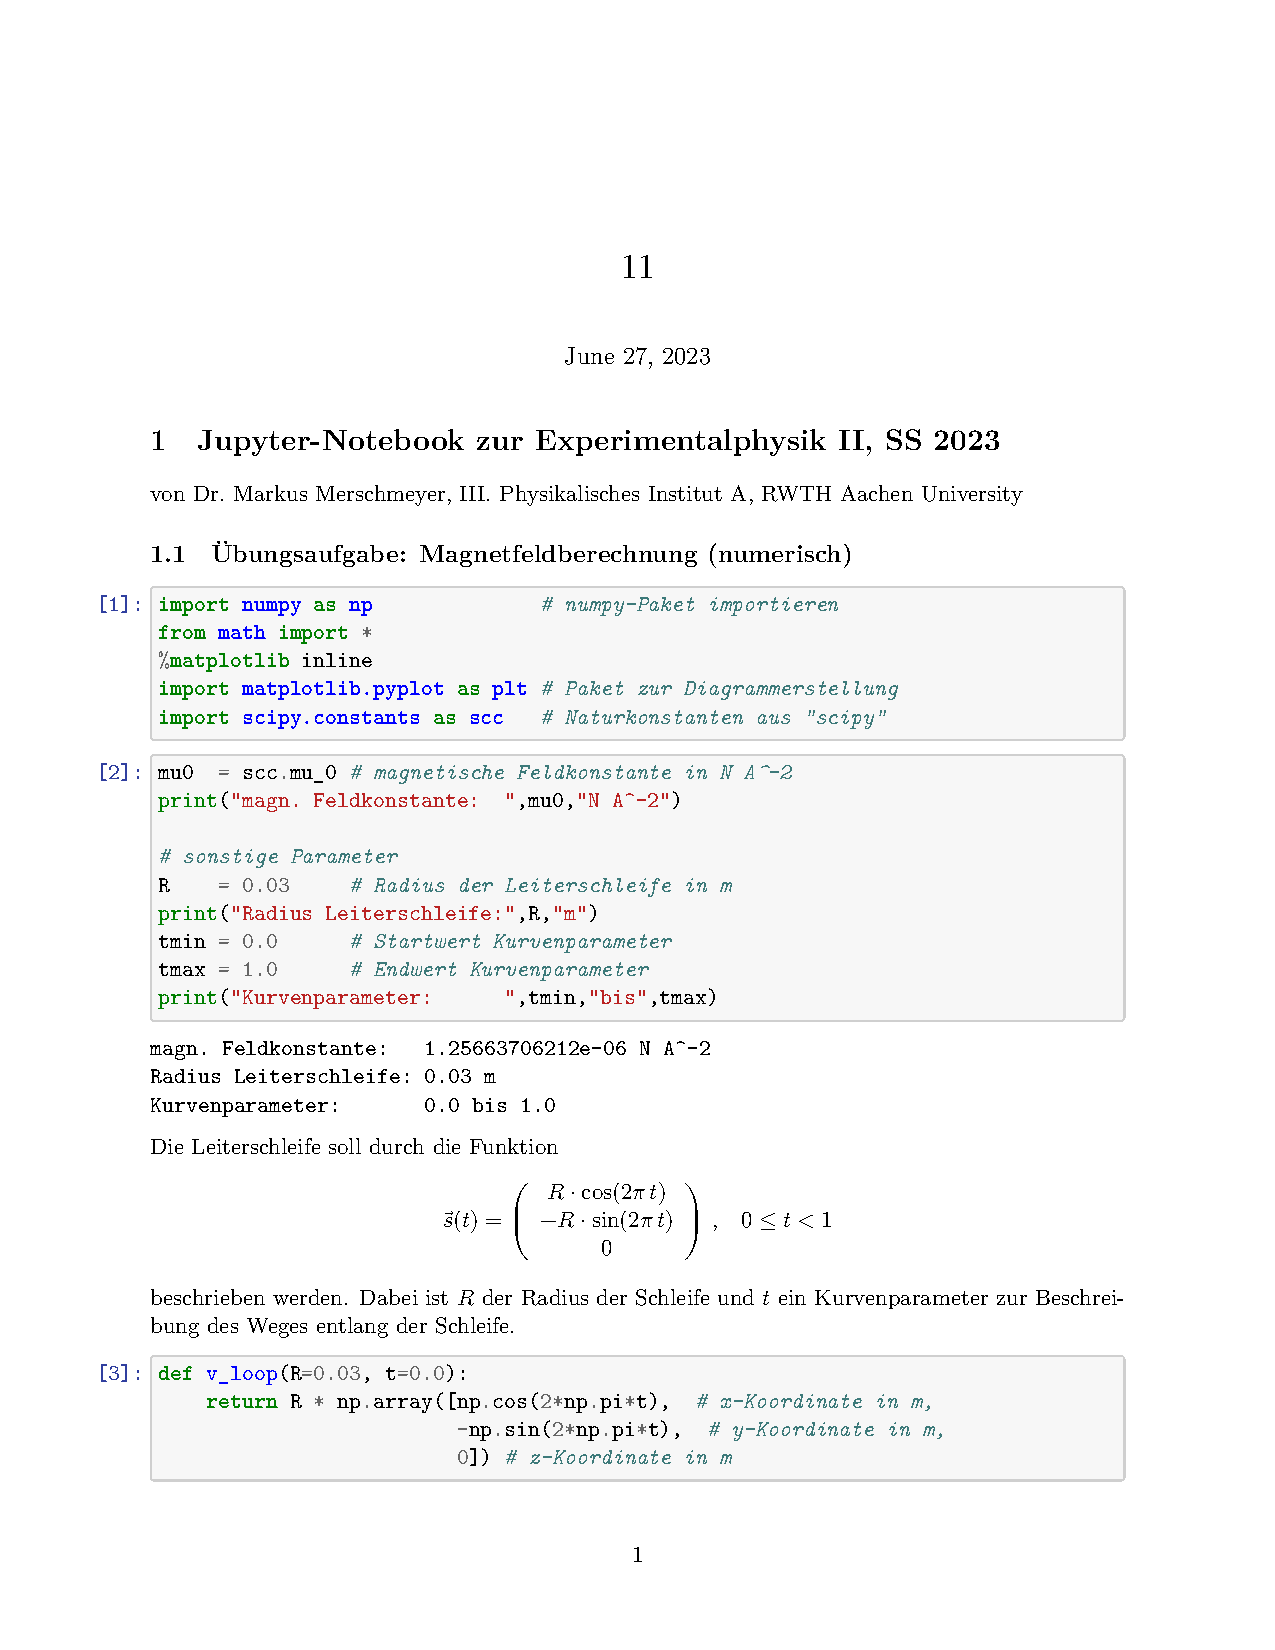
\includepdf[pages=-]{jupyter.pdf}
\end{document}